% Provenance (never printed): old terminale S material on magmatism in
% subduction zones (volcanic arcs above the slab, water released by the slab
% and hydrous melting of the mantle wedge, andesitic volcanism and granitoid
% plutons, growth of the continental crust). Owner (Sync 0): volcanic arc,
% hydrous melting, granodiorite, batholith, continental growth. Subduction,
% slab, Wadati-Benioff zone, blueschist and eclogite are g11.06's; partial and
% decompression melting and peridotite g11.05's; andesite, diorite, rhyolite,
% pluton g11.08's; continental crust g12.01's; magma, explosive eruption Book 1's
% (g7): recalled, never redefined. Figures: figdata/grade-12/arc_magmatism.py
% (GVP volcanoes, ComCat NE Japan band, dry solidus via grade-11
% geotherm_solidus.py, wet solidus brackets of Wang 2020 and Kawamoto-Holloway 1997).
\chapter{俯冲带的岩浆作用}\label{ch:g12:subduction-magmatism}

1980 年 5 月 18 日上午 8 时 32 分，一次震级 5.1 的地震
撼动了圣海伦斯火山。火山北侧坡体此前每天向外隆起约 2 米，
随即滑落，形成有记录以来规模最大的碎屑崩滑，
体积约 \qty{2.5}{km^3} 的岩石。失去上覆载荷后，
内部富含气体的岩浆沿侧向从滑坡缺口喷出，速度不低于
\qty{480}{km/h}，夷平了 \qty{600}{km^2} 范围内的森林。
15 分钟内，火山灰柱升高到超过 \qty{24}{km}，
喷发持续了 9 小时。61 人遇难或失踪。
% ledger: usgs:b2-msh-1980, usgs:msh-deaths

\begin{omfigure}
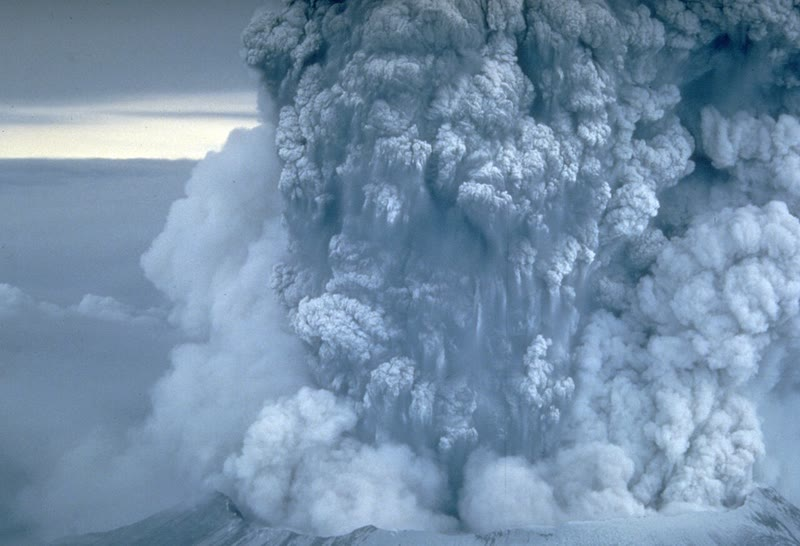
\includegraphics[width=0.55\linewidth]{images/book2/g12-swanson-st-helens-plume.jpg}

{\small 1980 年 5 月 18 日圣海伦斯火山的火山灰柱，
在不到 15 分钟内升至超过 \qty{24}{km}。照片：Donald
A. Swanson，USGS（公有领域）。}
\end{omfigure}
% ledger: photo:g12-st-helens, usgs:b2-msh-1980

圣海伦斯火山是一列火山中的一座——贝克山、雷尼尔山、胡德山、
夏斯塔山等——它们位于一块小型大洋板块\omterm{def:g11:subduction-zones:subduction}{俯冲}之处的上方，
即胡安·德福卡板块，它\omterm{def:g11:subduction-zones:subduction}{俯冲}到北美洲之下。本章探讨三个问题：
这些火山为何出现在那里，它们的喷发为何往往如此猛烈，
以及那些未能到达地表的岩浆去了哪里。
% ledger: earle:cascades

\begin{recall}
在\omterm{def:g11:subduction-zones:subduction}{俯冲带}，\omterm{def:g11:ocean-ridges:oceanic-lithosphere}{大洋岩石圈}板块沉回
另一板块之下的地幔中；其地震带即\omterm{def:g11:subduction-zones:benioff}{和达–贝尼奥夫带}，
沿\omterm{def:g11:subduction-zones:slab}{板片}向下延伸，深度可达 \qty{670}{km}
（见\cref{ch:g11:subduction-zones}）。地幔由\omterm{def:g11:ocean-ridges:peridotite}{橄榄岩}构成，它是固态的，
但上升且受压减弱的岩石可能\omterm{def:g11:ocean-ridges:partial-melting}{部分熔融}，
即\omterm{def:g11:ocean-ridges:partial-melting}{减压熔融}，如洋脊之下的情形（见\cref{ch:g11:ocean-ridges}）。
\omterm{def:g11:igneous-rocks:rock-names}{安山岩}是介于玄武岩与\omterm{def:g11:igneous-rocks:rock-names}{流纹岩}之间的\omterm{def:g11:igneous-rocks:volcanic-plutonic}{火山岩}，\omterm{def:g11:igneous-rocks:rock-names}{闪长岩}是其\omterm{def:g11:igneous-rocks:volcanic-plutonic}{深成岩}对应物，
\omterm{def:g11:igneous-rocks:intrusion}{深成岩体}则是在地下冷却的大规模岩浆体
（见\cref{ch:g11:igneous-rocks}）。\omterm{def:g12:continental-crust:continental-crust}{大陆地壳}厚而轻，
上部主要为花岗质岩石（见\cref{ch:g12:continental-crust}）。爆炸式
喷发借助岩浆自身的气体将其炸成碎块（第 1 册，七年级）。
\end{recall}
% ledger: tulane:magma-types, tulane:intrusions, rg14:crust

\section{火山弧}

陆地上的活火山大多并非随机分布。在自上一次冰期结束以来喷发过、
并被全球火山计划目录收录的 1214 座火山中，
有 838 座——超过三分之二——位于\omterm{def:g11:subduction-zones:subduction}{俯冲带}之上。
环绕太平洋的这些火山几乎连成一圈不间断的环带，
常被称为“火环”。其中每一条火山线都与海沟平行，
且位于不\omterm{def:g11:subduction-zones:subduction}{俯冲}的那一侧板块上。
% values: n_volcanoes 1214, n_subduction 838, frac_subduction 0.690 (arc_magmatism.py)
% ledger: data:gvp, tulane:arc

\begin{omfigure}
\begin{tikzpicture}
\begin{axis}[ommap, width=\linewidth, xtick={-180,-90,...,180}, ytick={-60,0,60},
  legend style={font=\scriptsize, at={(0.5,-0.13)}, anchor=north, legend columns=3,
    /tikz/every even column/.append style={column sep=6pt}}]
\addplot[fill=omLithAlluv, draw=black!45, line width=0.2pt, forget plot] table {figdata/out/shared-geo-land.dat};
\addplot[black!70, line width=0.5pt, forget plot] table {figdata/out/shared-geo-school-subduction.dat};
\addplot[fill=black!70, draw=none, forget plot] table {figdata/out/shared-geo-school-teeth.dat};
% computed in figdata/grade-12/arc_magmatism.py; ledger: data:gvp, data:pb2002, data:ne-land
\addplot[only marks, mark=triangle*, mark size=1.1pt, black!40] table[x=lon, y=lat] {figdata/out/grade-12-arc_magmatism-world-other.dat};
\addplot[only marks, mark=triangle*, mark size=1.3pt, omThm] table[x=lon, y=lat] {figdata/out/grade-12-arc_magmatism-world-sub.dat};
\addlegendimage{black!70, line width=0.5pt}
\legend{{其他火山}, {位于俯冲带之上的火山}, {海沟}}
\end{axis}
\end{tikzpicture}

{\small 自上一次冰期结束以来的活火山，位于\omterm{def:g11:subduction-zones:subduction}{俯冲带}之上者以红色标出，
并标出海沟（黑线，三角形
位于上覆板块一侧）。数据：史密森尼学会全球火山计划；
板块边界据 Bird（2003）；陆地数据来自 Natural Earth。}
\end{omfigure}
% values: n_subduction 838 of 1214 (arc_magmatism.py)

\begin{definition}[火山弧]\label{def:g12:subduction-magmatism:arc}
称\emph{火山弧}\index{火山弧}为\omterm{def:g11:subduction-zones:subduction}{俯冲带}上盘板块上与海沟平行的一列火山，
矗立于\omterm{def:g11:subduction-zones:slab}{板片}已达约一百千米深度处的上方。
当其从海底隆起时，为\emph{岛弧}，
如日本或印度尼西亚；位于大陆之上时，
则为大陆弧，
如安第斯山脉或喀斯喀特山脉。
\end{definition}
% ledger: tulane:arc, earle:arc-water, earle:cascades, sa06:slab-depth

离海沟最近的\omterm{def:g12:subduction-magmatism:arc}{火山弧}边缘称为\textbf{火山
前缘}：在其朝向海沟的一侧完全没有火山。
其下\omterm{def:g11:subduction-zones:slab}{板片}的深度有多大？

\begin{proposition}[火山前缘之下的板片]\label{prop:g12:subduction-magmatism:depth}
若\omterm{def:g11:subduction-zones:slab}{板片}为一平面，其相对于海沟的倾角为 $\theta$，且
火山前缘与海沟的水平距离为 $d$，则
\omterm{def:g11:subduction-zones:slab}{板片}顶面位于前缘之下，深度为
\[
  H = d \tan\theta .
\]
\end{proposition}

\begin{proof}
沿海沟作一竖直剖面。\omterm{def:g11:subduction-zones:slab}{板片}、地表以及
前缘正下方的竖直线构成一个直角三角形，
直角位于前缘正下方：沿地表的边为 $d$，
竖直边为 $H$，海沟处的角为 $\theta$。于是 $\tan\theta = H/d$。
\end{proof}

汇总了沿 \qty{33000}{km} 长岛弧的 839 个火山中心，
测得各中心之下的 $H$：按每段长 \qty{500}{km} 的弧段取平均，
其值介于 72 至 \qty{173}{km} 之间，平均为 \qty{105}{km}。
陡倾\omterm{def:g11:subduction-zones:slab}{板片}之上的岛弧靠近海沟，缓倾\omterm{def:g11:subduction-zones:slab}{板片}之上的岛弧
则远离海沟，但其下\omterm{def:g11:subduction-zones:slab}{板片}始终
深约一百千米。
% ledger: sa06:slab-depth

\begin{method}[寻找火山之下的板片]\label{met:g12:subduction-magmatism:slab}
\begin{enumerate}
  \item 取穿过岛弧的一条窄带中的地震，
        按真实比例，以深度对横向距离作图。
  \item 保留深于约 \qty{70}{km} 的地震：较浅的
        也会发生在上覆板块内，以及两板块间的
        断层上。
  \item 在火山前缘之下，画出深部地震的拟合线或读取其深度：
        此即该处\omterm{def:g11:subduction-zones:slab}{板片}的深度。
  \item 用 $H = d\tan\theta$ 进行校验，其中 $d$ 由海沟量起，
        倾角 $\theta$ 在剖面上量取。
\end{enumerate}
\end{method}

\begin{omfigure}
\begin{tikzpicture}
\begin{axis}[omsection, name=jp, scale only axis, width=0.8\linewidth, height=0.2857\linewidth,
  xmin=0, xmax=700, ymin=0, ymax=250, y dir=reverse,
  xlabel={距东经 \ang{138} 以东的距离（\unit{km}）}, ylabel={深度（\unit{km}）},
  xtick={0,100,...,700}, ytick={0,50,...,250}, tick label style={font=\small},
  every axis label/.append style={font=\small}]
% computed in figdata/grade-12/arc_magmatism.py; ledger: data:b2-usgs-ne-japan, data:gvp, data:pb2002
\addplot[only marks, mark=*, mark size=0.55pt, black!35] table[x=x_km, y=depth] {figdata/out/grade-12-arc_magmatism-jp-quakes.dat};
\addplot[omDef, line width=0.9pt, dashed] table[x=x_km, y=depth] {figdata/out/grade-12-arc_magmatism-jp-slab.dat};
\addplot[only marks, mark=triangle*, mark size=2.6pt, omThm] table[x=x_km, y expr=-7] {figdata/out/grade-12-arc_magmatism-jp-volc.dat};
\draw[omThm, densely dotted, line width=0.8pt] (axis cs:259.2,0) -- (axis cs:259.2,98.2);
\fill[omThm] (axis cs:259.2,98.2) circle (1.6pt);
\coordinate (front) at (axis cs:259.2,-14);
\coordinate (trench) at (axis cs:528.9,-14);
\coordinate (H) at (axis cs:262,60);
\coordinate (slab) at (axis cs:95,228);
\draw[black, line width=0.9pt] (axis cs:528.9,-12) -- (axis cs:528.9,0);
\end{axis}
\node[font=\scriptsize, anchor=south, text=omThm] at (front) {火山前缘（岩手）};
\node[font=\scriptsize, anchor=south] at (trench) {日本海沟};
\node[font=\scriptsize, anchor=west, text=omThm, fill=white, inner sep=1pt] at (H) {\qty{98}{km}};
\node[font=\scriptsize, anchor=west, text=omDef, fill=white, inner sep=1pt] at (slab) {板片，倾角约 \ang{20}};
\end{tikzpicture}

{\small 日本东北部剖面，比例真实：
北纬 \ang{37.5} 至 \ang{40.5} 之间、1976--2025 年震级不小于 4.5 的地震（灰色），
同一地带的火山（红色三角形）以及对
深于 \qty{70}{km} 的地震所作的拟合线（蓝色虚线）。东经 \ang{141.5} 以东的浅源地震中，五分之二
发生于 2011 年，该年发生了三月的特大
地震。数据：USGS
地震目录；Smithsonian Global Volcanism Program；板块边界
据 Bird（2003）。}
\end{omfigure}
% values: shallow (<70 km) events east of 141.5 E: 3622, of which 1451 in 2011 (0.40); ledger usgs:tohoku
% values: jp_front_lon 141.0 (x 259.2 km), jp_trench_lon 144.12 (x 528.9), jp_front_trench_km 269.4, jp_dip_deg 19.98, jp_H_geom 98.0, bin_141_median 98.15, jp_slab_depth_front 105.6 (arc_magmatism.py)

\begin{example}[日本东北部]\label{ex:g12:subduction-magmatism:japan}
图中该地带最东端的火山为岩手火山，位于东经 \ang{141.0}，
日本海沟位于东经 \ang{144.1}。该处经度一度的长度为
$111.2\cos\ang{39} \approx \qty{86.4}{km}$，故 $d \approx 3.12 \times 86.4
\approx \qty{270}{km}$。深部地震倾角约 \ang{20}，于是
\[
  H = 270 \times \tan\ang{20} \approx \qty{98}{km}.
\]
位于前缘正下方、深于 \qty{70}{km} 的地震，
其深度中位数为 \qty{98}{km}，二者吻合，接近世界
平均值。
\end{example}
% values: km_per_deg_lon 86.415, jp_front_trench_km 269.4, jp_dip_deg 19.98, jp_H_geom 97.98, bin_141_median 98.15 (arc_magmatism.py)

\section{水使地幔熔融}

岛弧之下，\omterm{def:g11:subduction-zones:slab}{板片}是冷的，其上的\omterm{def:g11:ocean-ridges:oceanic-lithosphere}{洋壳}也是冷的：
它无法熔化。岩浆必定来自\omterm{def:g11:subduction-zones:slab}{板片}之上的热地幔，即
\textbf{地幔楔}。但地幔楔并不上升，因此不能像洋脊之下那样
靠减压而熔化。另有一物能降低其熔化
温度：水。
% ledger: earle:settings (subducted crust stays cool), earle:flux-melting, earle:arc-water

\omterm{def:g11:ocean-ridges:oceanic-lithosphere}{洋壳}在形成处附近的洋脊一带浸满海水，
其中大量的水最终被锁在矿物之中，尤以
蛇纹石为最，蛇纹石由\omterm{def:g11:ocean-ridges:oceanic-lithosphere}{洋壳}的橄榄石和辉石形成。\omterm{def:g11:subduction-zones:slab}{板片}
下沉并变暖，这些矿物分解，释放出水。
水上升，进入其上方地幔楔的热\omterm{def:g11:ocean-ridges:peridotite}{橄榄岩}之中。
% ledger: earle:arc-water, tulane:arc

\begin{definition}[含水熔融]\label{def:g12:subduction-magmatism:hydrous-melting}
称\emph{含水熔融}\index{含水熔融}（亦称助熔）为
因加水而发生的岩石\omterm{def:g11:ocean-ridges:partial-melting}{部分熔融}，所加入的水使
岩石开始熔融的温度降低。
\end{definition}
% ledger: earle:flux-melting, earle:arc-water

在给定压强下，岩石开始熔化的温度即其
\textbf{固相线}。干\omterm{def:g11:ocean-ridges:peridotite}{橄榄岩}的固相线已广为人知；含水时则
难以测定，已发表的数值仍相差 200 至
\qty{600}{\celsius}。最新实验表明，在 950 至
\qty{1000}{\celsius} 之间，压强 \qty{3}{GPa}（约深 \qty{95}{km}）处，
固相线在 \qty{5}{GPa} 至 \qty{11}{GPa} 之间略高于 \qty{1000}{\celsius}。干\omterm{def:g11:ocean-ridges:peridotite}{橄榄岩}在 \qty{3}{GPa}
下，约在 \qty{1470}{\celsius} 才开始熔化：水使固相线
降低约 \qty{500}{\celsius}。
% values: dry_T_3gpa 1473.4, dry_minus_wet_3gpa 498, z_3gpa_km 95.2, dry_minus_wet_5gpa 658 (arc_magmatism.py)
% ledger: hirschmann:solidus, wang20:wet-solidus, kh97:wet-solidus, data:prem, earth:gmean

\begin{omfigure}
\begin{tikzpicture}
\begin{axis}[omrecord, name=sol, scale only axis, width=0.62\linewidth, height=6.2cm,
  xmin=700, xmax=1900, ymin=0, ymax=230, y dir=reverse,
  xlabel={温度 (\unit{\celsius})}, ylabel={深度 (\unit{km})},
  xtick={800,1000,...,1800}, ytick={0,50,...,200}, axis y line*=left]
% computed in figdata/grade-12/arc_magmatism.py (dry: Hirschmann 2000 with PREM pressures; wet: Wang 2020, Kawamoto-Holloway 1997)
\addplot[omProp, line width=1.2pt] table[x=T_dry, y=depth_km] {figdata/out/grade-12-arc_magmatism-solidus.dat};
\addplot[omDef, line width=2.4pt] coordinates {(950,95.24) (1000,95.24)};
\addplot[omDef, line width=1.2pt] coordinates {(1000,155.6) (1000,216.3)};
\draw[-{Stealth}, black!70, line width=0.8pt] (axis cs:1460,95.24) -- (axis cs:1015,95.24);
\coordinate (gap) at (axis cs:1240,95.24);
\coordinate (dry) at (axis cs:1600,40);
\coordinate (wet) at (axis cs:1015,190);
\coordinate (wet3) at (axis cs:975,90);
\end{axis}
\begin{axis}[scale only axis, width=0.62\linewidth, height=6.2cm, at={(sol.south west)}, anchor=south west,
  xmin=700, xmax=1900, ymin=0, ymax=230, y dir=reverse, axis x line=none, axis y line*=right,
  axis line style={-}, ylabel={压强 (\unit{GPa})},
  ytick={34.9,65.1,95.2,125.5,155.6,185.9,216.3}, yticklabels={1,2,3,4,5,6,7},
  every axis label/.append style={font=\small}, tick label style={font=\small}]
% pressure ticks at the PREM depths of 1-7 GPa (arc_magmatism.depth_at_pressure)
\end{axis}
\node[font=\scriptsize, anchor=south] at ([yshift=2pt]gap) {约 \qty{500}{\celsius}};
\node[font=\scriptsize, text=omProp, anchor=west, align=left] at (dry) {干橄榄岩 \\开始熔化};
\node[font=\scriptsize, text=omDef, anchor=west, align=left] at (wet) {含水时：略高于 \\\qty{1000}{\celsius}};
\node[font=\scriptsize, text=omDef, anchor=south] at ([yshift=2pt]wet3) {950--1000};
\end{tikzpicture}

{\small 地幔\omterm{def:g11:ocean-ridges:peridotite}{橄榄岩}开始熔化的温度与
深度的关系：干燥（橙色）与\omterm{def:g10:why-clouds-form:humidity}{饱和}含水（蓝色，迄今测得的两个范围）
在岛弧下方\omterm{def:g11:subduction-zones:slab}{板片}的深度，约 \qty{100}{km} 处，水
使其降低约 \qty{500}{\celsius}。来源：Hirschmann（2000），采用
PREM 密度；Wang 等（2020）；Kawamoto 与 Holloway（1997）。}
\end{omfigure}
% values: dry_T_3gpa 1473.4, dry_T_100km 1489.4, P_100km_gpa 3.157 (arc_magmatism.py)

因此，水所起的作用是加热本身无法实现的：它使部分炽热的
楔形地幔熔融。岩浆比周围固态地幔轻，向上
\omterm{def:g11:fossil-fuel-geology:migration}{运移}至地表：一部分喷发，更多的留在地下冷却。
水被释放之处，以及其上楔体温度足以在含水后熔融之处，
正是决定火山前缘位于\omterm{def:g11:subduction-zones:slab}{板片}上方
约一百千米处的因素。
% ledger: earle:arc-water, tulane:arc, sa06:slab-depth, wang20:wet-solidus (position of the volcanic front controlled by melting in the wedge)

\begin{omfigure}
\begin{tikzpicture}[x=1cm, y=1cm, font=\scriptsize]
  % mantle
  \fill[omLithPeridotite!45] (0,-0.9) -- (7.4,-0.9) -- (7.5,-0.85) -- (6.5,-1.6) -- (5.5,-2.6) -- (4.5,-3.8)
    -- (4.25,-4.3) -- (0,-4.3) -- cycle;
  % sea and overriding continental crust
  \fill[omSea] (8.0,0) -- (12,0) -- (12,-0.4) -- (8.5,-0.4) -- cycle;
  \fill[omLithGranite!55] (0,0.1) -- (8.0,0.1) -- (8.5,-0.4) -- (7.5,-0.85) -- (7.4,-0.9) -- (0,-0.9) -- cycle;
  % the slab
  \fill[omLithBasalt!45, draw=black!60] (12,-0.4) -- (8.5,-0.4) -- (7.5,-0.85) -- (6.5,-1.6) -- (5.5,-2.6) -- (4.5,-3.8)
    -- (4.25,-4.3) -- (5.15,-4.3) -- (5.2,-4.3) -- (6.15,-3.15) -- (7.1,-2.2) -- (8.0,-1.55) -- (8.9,-1.2) -- (12,-1.2) -- cycle;
  \node at (10.4,-0.8) {大洋岩石圈};
  \node[anchor=west] at (6.0,-3.4) {下沉的板片};
  % melting in the wedge, rising magma, plutons, volcano
  \fill[omThm!35, draw=omThm, densely dashed] (5.2,-1.75) ellipse (0.6 and 0.3);
  \node[omThm] at (5.2,-1.75) {熔融};
  \foreach \y in {-1.3,-1.05} \fill[omThm!80] (5.2,\y) circle (0.07);
  \fill[omLithGranite, draw=black!60] (4.75,-0.55) ellipse (0.42 and 0.2);
  \fill[omLithGranite, draw=black!60] (5.65,-0.4) ellipse (0.32 and 0.16);
  \node[anchor=east] at (4.25,-0.55) {深成岩体};
  \draw[omThm, line width=1pt] (5.2,0.1) -- (5.2,-0.85);
  \fill[black!65] (4.75,0.1) -- (5.2,0.75) -- (5.65,0.1) -- cycle;
  \node[anchor=south] at (5.2,0.8) {火山};
  % water released by the slab
  \foreach \x/\y in {6.5/-1.6, 6.0/-2.1, 5.6/-2.5}
    \draw[omDef, -{Stealth}, line width=0.7pt, decorate, decoration={snake, amplitude=0.6pt, segment length=4pt, post length=1.5mm}]
      (\x,\y) -- ++(-0.3,0.3);
  \draw[omDef, line width=0.3pt] (7.5,-2.75) -- (6.35,-2.0);
  \node[omDef, anchor=west, align=left] at (7.5,-2.75) {水由板片 \\释放};
  % labels and depth scale
  \node at (1.8,-0.4) {陆壳};
  \node[black!70, align=center] at (2.3,-3.6) {炽热的地幔楔 \\（橄榄岩）};
  \node[anchor=south] at (8.5,0.12) {海沟};
  \draw[black!60, |-|] (0.4,0.1) -- node[left, align=right] {约 \\\qty{100}{km}} (0.4,-2.96);
  \draw[black!45, densely dotted] (0.4,-2.96) -- (5.2,-2.96);
  \fill[black!70] (5.2,-2.96) circle (1.3pt);
  \draw[black!45, densely dotted] (5.2,-2.96) -- (5.2,-2.05);
\end{tikzpicture}

{\small \omterm{def:g11:subduction-zones:subduction}{俯冲带}的岩浆作用（示意图，未按比例绘制）。\omterm{def:g11:subduction-zones:slab}{板片}
升温后，其中的矿物释出水分，水向上进入炽热的地幔
楔，使其\omterm{def:g11:ocean-ridges:partial-melting}{部分熔融}。岩浆上升：一部分在火山处喷发，
更多的则在地壳中冷却形成\omterm{def:g11:igneous-rocks:intrusion}{深成岩体}。}
\end{omfigure}
% ledger: earle:arc-water, earle:flux-melting, tulane:arc, tulane:ridge-rocks, sa06:slab-depth

\section{安山岩与花岗闪长岩}

含水\omterm{def:g11:ocean-ridges:peridotite}{橄榄岩}最初生成的熔体并非玄武质。在
\qty{1}{GPa}下的实验中，水\omterm{def:g10:why-clouds-form:humidity}{饱和}的\omterm{def:g11:ocean-ridges:peridotite}{橄榄岩}所生成的熔体为
岩浆在岛弧厚厚的地壳中上升，冷却时成分也随之改变，
由玄武质向安山质和流纹质演化。因此，弧岩浆
比洋脊玄武岩富含二氧化硅——安山质岩浆
含有 55 至 \qty{65}{\percent} 的二氧化硅——并携带着
促成其生成的水。
% ledger: kh97:wet-solidus (andesitic melts at 1 GPa), tulane:eruptions, tulane:ridge-rocks, tulane:magma-types

这两种性质都使其喷发十分猛烈。岩浆所含二氧化硅越多，
其黏度越大，气体越难逸出；爆炸式
喷发在气体含量高、黏度大时更易发生，如
安山质和流纹质岩浆。几乎所有复式火山都位于
\omterm{def:g11:subduction-zones:subduction}{俯冲带}之上：锥体高达数千米，直径可达 \qty{20}{km}，
坡度为 10 至 30 度，喷发形式从平静的熔岩流动到爆炸不等。
圣海伦斯火山之下，宽约 \qty{1}{km} 的岩浆房
自地下约 6 至 \qty{14}{km} 深处延伸。
% ledger: tulane:magma-types, tulane:eruptions, earle:composite

多数弧岩浆从未喷发。它在地壳中缓慢冷却，结晶成
粗粒岩石。

\begin{definition}[花岗闪长岩]\label{def:g12:subduction-magmatism:granodiorite}
\emph{花岗闪长岩}\index{花岗闪长岩}是一种粗粒\omterm{def:g11:igneous-rocks:volcanic-plutonic}{深成岩}，
与花岗岩相似，但斜长石多于钾长石：石英占浅色矿物的 20 至
\qty{60}{\percent}，斜长石占其长石的 65 至
\qty{90}{\percent}；它常含黑云母
或角闪石。
\end{definition}
% ledger: bgs:granodiorite

\begin{omfigure}
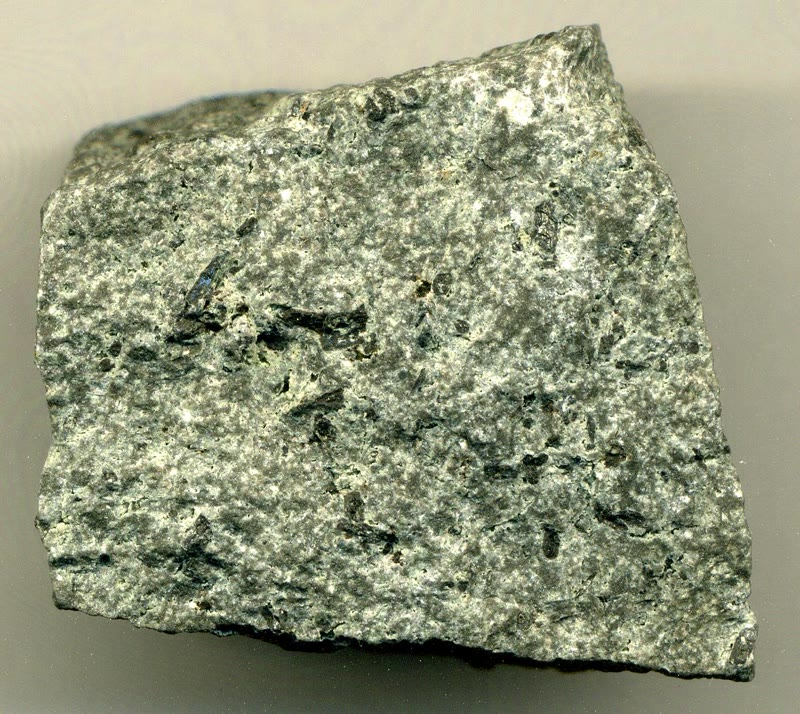
\includegraphics[height=4.4cm]{images/book2/g12-stjohn-andesite.jpg}\hspace{0.03\linewidth}%
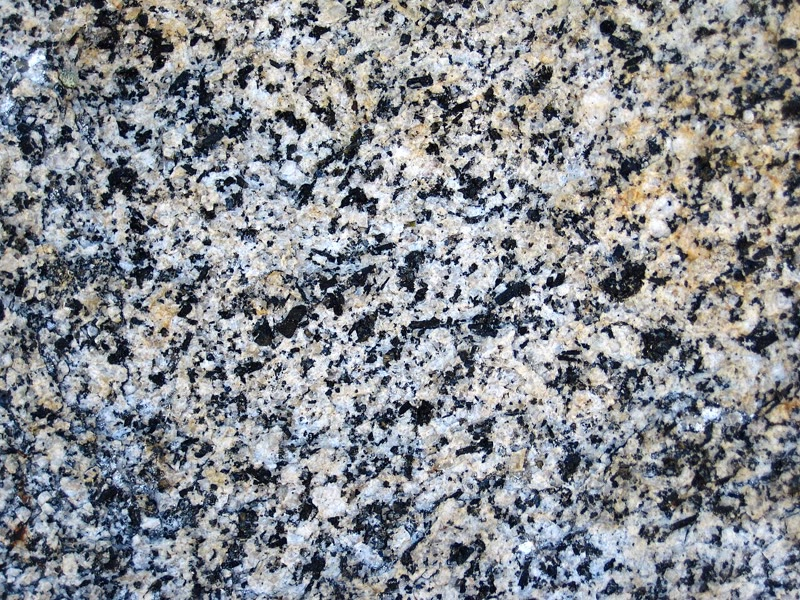
\includegraphics[height=4.4cm]{images/book2/g12-stjohn-granodiorite.jpg}

{\small 左：\omterm{def:g11:igneous-rocks:rock-names}{安山岩}，弧区的一种细粒\omterm{def:g11:igneous-rocks:volcanic-plutonic}{火山岩}。右：
内华达山脉的\omterm{def:g12:subduction-magmatism:granodiorite}{花岗闪长岩}，含白色斜长石、灰色石英和
黑色的黑云母与角闪石。照片：James St.~John（CC~BY~2.0）。}
\end{omfigure}
% ledger: photo:g12-andesite, photo:g12-granodiorite

平均而言，上陆壳约含 \qty{67}{\percent}
\ce{SiO2}，属\omterm{def:g11:igneous-rocks:felsic-mafic}{长英质}，与弧区在其\omterm{def:g12:subduction-magmatism:batholith}{岩基}中大量
形成的花岗岩相似。
% ledger: rg14:crust (upper crust SiO2 66.6 wt %), tulane:magma-types, tulane:intrusions

\begin{definition}[岩基]\label{def:g12:subduction-magmatism:batholith}
\emph{岩基}\index{岩基}是一大块\omterm{def:g11:igneous-rocks:volcanic-plutonic}{深成岩}，其经侵蚀后出露的面积
超过 \qty{100}{km^2}。它形成于多个先后侵入的
\omterm{def:g11:igneous-rocks:intrusion}{深成岩体}在地表之下相连。
\end{definition}
% ledger: earle:batholith, tulane:intrusions

世界最大的\omterm{def:g12:subduction-magmatism:batholith}{岩基}之一，海岸\omterm{def:g11:igneous-rocks:volcanic-plutonic}{深成岩}群沿
太平洋海岸延伸，从加拿大西部温哥华地区
直至阿拉斯加东南部。加利福尼亚的内华达\omterm{def:g12:subduction-magmatism:batholith}{岩基}形成于
\omterm{def:g11:subduction-zones:subduction}{俯冲带}之上；其中优胜美地的花岗岩大多在白垩纪结晶，
距今 1.05 亿至 8500 万年前。其上覆岩石在数百万年间被剥蚀，
深处冷却的\omterm{def:g11:igneous-rocks:intrusion}{深成岩体}如今构成
山脉。
% ledger: earle:batholith, nps:yosemite, photo:g12-sierra-nevada (St. John description), ics:base.Cretaceous

\begin{omfigure}
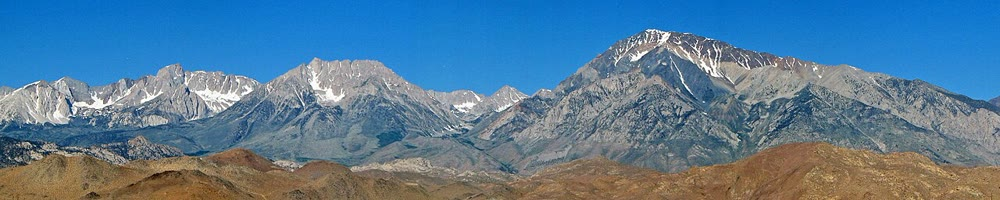
\includegraphics[width=0.94\linewidth]{images/book2/g12-stjohn-sierra-nevada-batholith.jpg}

{\small 自东侧望去的内华达山脉：内华达\omterm{def:g12:subduction-magmatism:batholith}{岩基}的花岗岩与
\omterm{def:g12:subduction-magmatism:granodiorite}{花岗闪长岩}，在白垩纪于\omterm{def:g11:subduction-zones:subduction}{俯冲带}上方的深处结晶。
照片：James St.~John
（CC~BY~2.0）。}
\end{omfigure}
% ledger: photo:g12-sierra-nevada, nps:yosemite

\section{大陆如何增生}

\begin{definition}[大陆增生]\label{def:g12:subduction-magmatism:continental-growth}
\emph{大陆增生}\index{大陆增生}是指新增的\omterm{def:g12:continental-crust:continental-crust}{大陆地壳}，
由地幔物质形成，主要通过弧区岩浆作用实现。
大陆的净增生量等于上述增加量减去
返回地幔的\omterm{def:g12:continental-crust:continental-crust}{大陆地壳}。
\end{definition}
% ledger: sv09:growth, ss09:balance

弧区是大陆轻质岩石的形成之处。据估计，当今弧区
每年增加的岩浆量在岛弧约为 \qty{1.5}{km^3}，
在大陆弧约为每年 \qty{1.0}{km^3}；长期平均
约为每年 \qty{2.7}{km^3}。但\omterm{def:g11:subduction-zones:subduction}{俯冲带}也会把\omterm{def:g12:continental-crust:continental-crust}{大陆地壳}
带回地幔：随\omterm{def:g11:subduction-zones:slab}{板片}下沉的沉积物，以及从上盘板块底部
刮落的碎片，约每年 \qty{3.2}{km^3}。两者相近，
过去数亿年间大陆的净增生量
或许接近于零，甚至为负。
% ledger: sv09:growth, ss09:balance

大陆还会以另一种方式在边缘生长。\omterm{def:g12:continental-crust:continental-crust}{大陆地壳}过于
轻，难以\omterm{def:g11:subduction-zones:subduction}{俯冲}，因此当板块把大陆带入海沟时，
两块大陆在碰撞中焊接在一起
（见\cref{ch:g12:mountain-building}）。每块大陆都有一个古老的核心，即\omterm{def:g12:continental-crust:craton}{克拉通}，
周围环绕着较年轻的岩石带，即早先造山带\omterm{def:g12:mountain-building:fold}{褶皱}变形的根部，
这些岩带先后在其边缘增生而成
（见\cref{ch:g12:continental-crust}）。
% ledger: tulane:no-subduct (continental crust too buoyant to subduct), earle:collision, tulane:cratons

\section{练习}

\begin{exercise}[$\star$]\label{exo:g12:subduction-magmatism:1}
写出下列描述所对应的术语：(a) 与海沟平行、位于不\omterm{def:g11:subduction-zones:subduction}{俯冲}一侧板块上的火山链；
(b) 向岩石中加水引起的熔融；(c) 一种\omterm{def:g11:igneous-rocks:volcanic-plutonic}{深成岩}，其
斜长石多于钾长石，且石英含量多于
\qty{20}{\percent}；(d) 面积大于
\qty{100}{km^2} 的\omterm{def:g11:igneous-rocks:intrusion}{深成岩体}；(e) 由地幔物质形成的
新\omterm{def:g12:continental-crust:continental-crust}{大陆地壳}的增生。
\end{exercise}

\begin{exercise}[$\star$]\label{exo:g12:subduction-magmatism:2}
1980 年 5 月 18 日，圣海伦斯火山的火山灰柱上升了超过 \qty{24}{km}
在不到 15 分钟的时间内。(1) 其平均上升速度的最小值是多少，分别以
\unit{km/h} 和 \unit{m/s} 表示？(2) 将其与侧向爆炸的速度相比较，
后者至少为 \qty{480}{km/h}。
\end{exercise}

\begin{exercise}[$\star$]\label{exo:g12:subduction-magmatism:3}
在自末次冰期结束以来仍活动的 1214 座火山名录中，
其中 838 座位于\omterm{def:g11:subduction-zones:subduction}{俯冲带}之上。(1) 这一比例是多少？(2) 这些火山
位于海沟的哪一侧？(3) 为什么在海沟与火山锋之间
没有火山？
\end{exercise}

\begin{exercise}[$\star$]\label{exo:g12:subduction-magmatism:4}
某粗粒岩石含石英 \qty{25}{\percent}，斜长石 \qty{45}{\percent}，
钾长石 \qty{15}{\percent}，黑云母与角闪石
共占 \qty{15}{\percent}。(1) 其长石中斜长石所占的比例是多少？
(2) 它是\omterm{def:g12:subduction-magmatism:granodiorite}{花岗闪长岩}吗？
\end{exercise}

\begin{exercise}[$\star$]\label{exo:g12:subduction-magmatism:5}
说出\omterm{def:g12:subduction-magmatism:arc}{火山弧}上的火山比洋脊火山
喷发更剧烈的两个原因。
\end{exercise}

\begin{exercise}[$\star\star$]\label{exo:g12:subduction-magmatism:6}
(1) 火山锋距海沟 \qty{150}{km}，其下\omterm{def:g11:subduction-zones:slab}{板片}
倾角为 \ang{35}。该处\omterm{def:g11:subduction-zones:slab}{板片}深度是多少？(2) 与
\qty{105}{km} 的平均值相比较。
\end{exercise}

\begin{exercise}[$\star\star$]\label{exo:g12:subduction-magmatism:7}
设\omterm{def:g11:subduction-zones:slab}{板片}在每个火山锋下方的深度均为 \qty{105}{km}，火山锋距海沟
多远？\omterm{def:g11:subduction-zones:slab}{板片}倾角分别为 \ang{20} 与
\ang{45} 时各为多少？这说明应在何处寻找\omterm{def:g12:subduction-magmatism:arc}{火山弧}？
\end{exercise}

\begin{exercise}[$\star\star$]\label{exo:g12:subduction-magmatism:8}
在 \qty{100}{km} 深处，压强约为 \qty{3.16}{GPa}。(1) 利用 $T =
-5.104P^2 + 132.9P + 1120.7$（$P$ 单位为 \unit{GPa}，$T$ 单位为 \unit{\celsius}），
计算该处干燥\omterm{def:g11:ocean-ridges:peridotite}{橄榄岩}开始熔融的温度。
(2) 有水时，约在 \qty{1000}{\celsius} 开始熔融。水使其
降低了多少？(3) 设该处地幔楔温度约为
\qty{1300}{\celsius}。它干燥时会熔融吗？含水时呢？
\end{exercise}

\begin{exercise}[$\star\star$]\label{exo:g12:subduction-magmatism:9}
圣海伦斯火山的碎屑崩塌移动了约 \qty{2.5}{km^3}
的岩石。\omterm{def:g12:subduction-magmatism:arc}{火山弧}每年增加约 \qty{2.7}{km^3} 的新地壳。(1) 这次崩塌
相当于全球\omterm{def:g12:subduction-magmatism:arc}{火山弧}岩浆作用多少天的产量？(2) 为何
这一比较只涉及规模问题？
\end{exercise}

\begin{exercise}[$\star\star$]\label{exo:g12:subduction-magmatism:10}
(1) 按每年 \qty{2.7}{km^3} 计，\omterm{def:g12:subduction-magmatism:arc}{火山弧}一百万年
共增加多少新地壳？(2) \omterm{def:g12:continental-crust:continental-crust}{大陆地壳}约有 \qty{9e9}{km^3}。
假如其中没有任何损失，仅靠\omterm{def:g12:subduction-magmatism:arc}{火山弧}形成这一体积需要多久？(3) 与
地球年龄 45 亿年相比较。
\end{exercise}

\begin{exercise}[$\star\star$]\label{exo:g12:subduction-magmatism:11}
(1) 在横跨日本的剖面中，拟合\omterm{def:g11:subduction-zones:slab}{板片}时为何舍去许多
浅于 \qty{70}{km} 的地震？(2) 深部地震在东经 \ang{140.5} 处
位于 \qty{116}{km} 深，在东经 \ang{141.5} 处位于 \qty{80}{km} 深，
每度经度对应 \qty{86.4}{km}。计算\omterm{def:g11:subduction-zones:slab}{板片}的倾角。
\end{exercise}

\begin{exercise}[$\star\star\star$]\label{exo:g12:subduction-magmatism:12}
证明：对于距海沟为 $d$、其上方\omterm{def:g11:subduction-zones:slab}{板片}倾角为
$\theta$ 的火山锋，从海沟沿\omterm{def:g11:subduction-zones:slab}{板片}量至火山锋下方
那一点的距离为 $d/\cos\theta$。对日本（$d = \qty{270}{km}$，
$\theta = \ang{20}$）而言，该距离是多少？太平洋板块以
约 \qty{83}{mm} 每年的速度向日本移动；若沿整个\omterm{def:g11:subduction-zones:slab}{板片}均取该速度，
一块海底从海沟运动到
火山下方需要多久？
\end{exercise}
% ledger: usgs:tohoku (83 mm/yr)

\begin{exercise}[$\star\star\star$]\label{exo:g12:subduction-magmatism:13}
圣海伦斯火山的岩浆房宽约 \qty{1}{km}，
自地下约 6 延伸至 \qty{14}{km} 深。(1) 将其视为竖直圆柱体，
估算其体积。(2) 与崩塌体的 \qty{2.5}{km^3} 相比较。
(3) 计算岩浆房顶部与底部的\omterm{def:g12:metamorphic-rocks:lithostatic}{静岩压力}（$\rho =
\qty{2830}{kg/m^3}$，$g = \qty{9.81}{m/s^2}$）。
\end{exercise}

\begin{exercise}[$\star\star\star$]\label{exo:g12:subduction-magmatism:14}
\omterm{def:g12:subduction-magmatism:arc}{火山弧}每年增加约 \qty{2.7}{km^3} 的地壳，而\omterm{def:g11:subduction-zones:subduction}{俯冲带}每年
约带回 \qty{3.2}{km^3}。(1) 每百万年的净变化量是多少？
(2) 在 5 亿年内，这一量占 \qty{9e9}{km^3} 地壳的
比例是多少？(3) 作者称此净增长“实际上可忽略不计”。
鉴于每个估计值的不确定度，为何可以这样说？
\end{exercise}

\begin{exercise}[$\star\star\star$]\label{exo:g12:subduction-magmatism:15}
一个\omterm{def:g12:subduction-magmatism:batholith}{岩基}暴露出 \qty{20000}{km^2} 的\omterm{def:g12:subduction-magmatism:granodiorite}{花岗闪长岩}，其\omterm{def:g11:igneous-rocks:intrusion}{深成岩体}
固结于地下 5 至 \qty{15}{km} 之间。(1) 估算其所代表的岩浆体积，
取其厚度为 \qty{10}{km}。(2) 全球所有大陆弧合计每年 \qty{1}{km^3} 的速率，
需要多久才能形成该\omterm{def:g12:subduction-magmatism:batholith}{岩基}？这说明
\omterm{def:g12:subduction-magmatism:batholith}{岩基}形成所经历的时间
有多长？
(3) 在其能被看到之前，上方须剥蚀掉多少岩石？
\end{exercise}

\begin{problem}[{周末问题——日本火山之下}]
\label{pb:g12:subduction-magmatism:1}
% ledger: data:b2-usgs-ne-japan, data:gvp, data:pb2002, sa06:slab-depth, hirschmann:solidus, wang20:wet-solidus, earle:arc-water, data:prem
% values (arc_magmatism.py): Megata 139.725, Iwate 141.001, trench 144.12; bins 140.5/141/141.5: 116.4/98.15/80.35 km; P_100km 3.157, dry_T_100km 1489
北纬 \ang{37.5} 至 \ang{40.5} 之间的日本东北部火山，
位于东经 \ang{139.7}（Megata，最西）与东经 \ang{141.0}（Iwate，最东）之间；
日本海沟位于东经 \ang{144.1}。表中给出 1976--2025 年间、
三个经度带内深于 \qty{70}{km} 的地震的中位深度。
纬度每度取 \qty{111.2}{km}。

\begin{center}
\small
\begin{tabular}{|l|c|c|c|}
\hline
经度（\unit{\degree}~E） & 140.5 & 141.0 & 141.5 \\ \hline
中位深度（\unit{km}） & 116 & 98 & 80 \\ \hline
\end{tabular}
\end{center}

\medskip
\noindent\textbf{第一部分——火山锋。}
\begin{enumerate}
  \item 证明北纬 \ang{39} 处经度每度约为
        \qty{86.4}{km}。
  \item 火山锋距海沟多远？
  \item \omterm{def:g12:subduction-magmatism:arc}{火山弧}从岩手至 Megata 的宽度是多少？
  \item 火山位于哪一块板块之上，
        位于海沟的哪一侧？
  \item 为什么海沟与岩手之间没有火山？
\end{enumerate}

\medskip
\noindent\textbf{第二部分——地震部分。}
\begin{enumerate}[resume]
  \item 中位深度由
        \ang{140.5} 变至东经 \ang{141.5}，变化了多少千米？
  \item 水平距离是多少？
  \item 计算\omterm{def:g11:subduction-zones:slab}{板片}的倾角。
  \item 将自东经 \ang{141.0}、\qty{98}{km} 处的直线延伸至
        地表，它在何处与地表相交？该处距海沟多远？
  \item 试说明为什么\omterm{def:g11:subduction-zones:slab}{板片}靠近海沟处比深处更平缓。
\end{enumerate}

\medskip
\noindent\textbf{第三部分——火山下方的\omterm{def:g11:subduction-zones:slab}{板片}。}
\begin{enumerate}[resume]
  \item 利用第 2 题的距离与
        \ang{20} 的倾角，计算 $H = d\tan\theta$。
  \item 将其与火山锋下方的中位深度进行比较。
  \item 将两者分别与全球范围 72 至 \qty{173}{km}，
        以及平均值 \qty{105}{km} 相比较。
  \item 利用第 9 题的直线，求 Megata 下方\omterm{def:g11:subduction-zones:slab}{板片}的深度是多少？
  \item 设\omterm{def:g12:subduction-magmatism:arc}{火山弧}地壳厚约 \qty{35}{km}，火山锋
        下方\omterm{def:g11:subduction-zones:slab}{板片}的顶部位于地壳还是地幔中？
        它位于地壳底面以下多远？
\end{enumerate}

\medskip
\noindent\textbf{第四部分——水的来源。}
\begin{enumerate}[resume]
  \item \omterm{def:g11:subduction-zones:slab}{板片}中的水在何处进入其岩石，
        大量的水保存在哪种矿物中？
  \item 在 \qty{100}{km} 深处，压强约为 \qty{3.16}{GPa}。
        用 $T = -5.104P^2 + 132.9P + 1120.7$ 计算此处的干固相线温度。
  \item 有水时，固相线介于 950 与 \qty{1000}{\celsius} 之间。
        水使固相线降低了多少？
  \item 为什么冷的\omterm{def:g11:subduction-zones:slab}{板片}本身不能作为岩浆的来源？
  \item 总结：日本东北部火山锋
        下方的\omterm{def:g11:subduction-zones:slab}{板片}深度是多少？
\end{enumerate}
\end{problem}
